\cleardoublepage                                  % 
\chapter{Discusion}
\label{cap:Discusion}

\section{Mediciones de corriente en cargas no lineales}
En los últimos años, la cantidad de dispositivos con cargas no lineales en entornos residenciales ha aumentado de manera significativa, impulsada principalmente por la masificación de dispositivos electrónicos basados en fuentes conmutadas, tales como computadoras, televisores, cargadores, iluminación LED y electrodomésticos modernos. En este contexto, resulta crucial que los sistemas de monitoreo energético sean capaces de medir correctamente este tipo de consumos, ya que constituyen una porción cada vez más representativa de la demanda total.

A diferencia de las cargas lineales, donde la corriente es proporcional a la tensión y mantiene una forma de onda senoidal, las cargas no lineales presentan corrientes altamente distorsionadas, con la presencia de armónicos y picos abruptos. 
Debido a que el cálculo RMS es válido para cualquier forma de onda, es posible utilizar el mismo método de cálculo para obtener una estimación de la corriente en condiciones no lineales.

Con el objetivo de analizar el comportamiento del sistema frente a cargas no lineales, se realizó una evaluación experimental utilizando como caso de estudio un cargador de computadora portátil, representativo de este tipo de consumos debido a su naturaleza conmutada. Este tipo de dispositivo presenta una corriente caracterizada por picos pronunciados y una alta distorsión respecto de la forma senoidal ideal, lo que lo convierte en un escenario adecuado para validar el desempeño del sistema de medición.

Durante el ensayo, se compararon los valores de corriente obtenidos por el sistema desarrollado con mediciones de referencia realizadas mediante una punta de corriente conectada a un osciloscopio. La La  punta  fue  ajustada  a  una  sensibilidad  de 100  $mV$/$A$,  obteniéndose  un  consumo  de  0,490  $A$  de  corriente eficaz como se observa en la Figura~\ref{fig:medicion_referencia}. 

\begin{figure}[htbp]
    \centering
    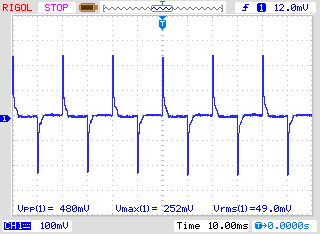
\includegraphics[width=0.8\textwidth]{imagenes/medicion_referencia.png}
    \caption{Medición de corriente en un cargador de computadora portátil utilizando la punta de corrriente conectada a un osciloscopio.}
    \label{fig:medicion_referencia}  
\end{figure}

El valor de corriente reportado por el sistema corresponde al nodo NC3, que al momento del ensayo tenía conectada la carga no lineal. En la Figura~\ref{fig:medicion_nc3} se presentan los resultados de una de las pruebas realizadas para la validación del sistema, donde puede observarse que el nodo informa un consumo de 0,492 $A$. Este valor presenta una diferencia de 2 $mA$ respecto de la medición obtenida mediante la punta de corriente.

\begin{figure}[htbp]
    \centering
    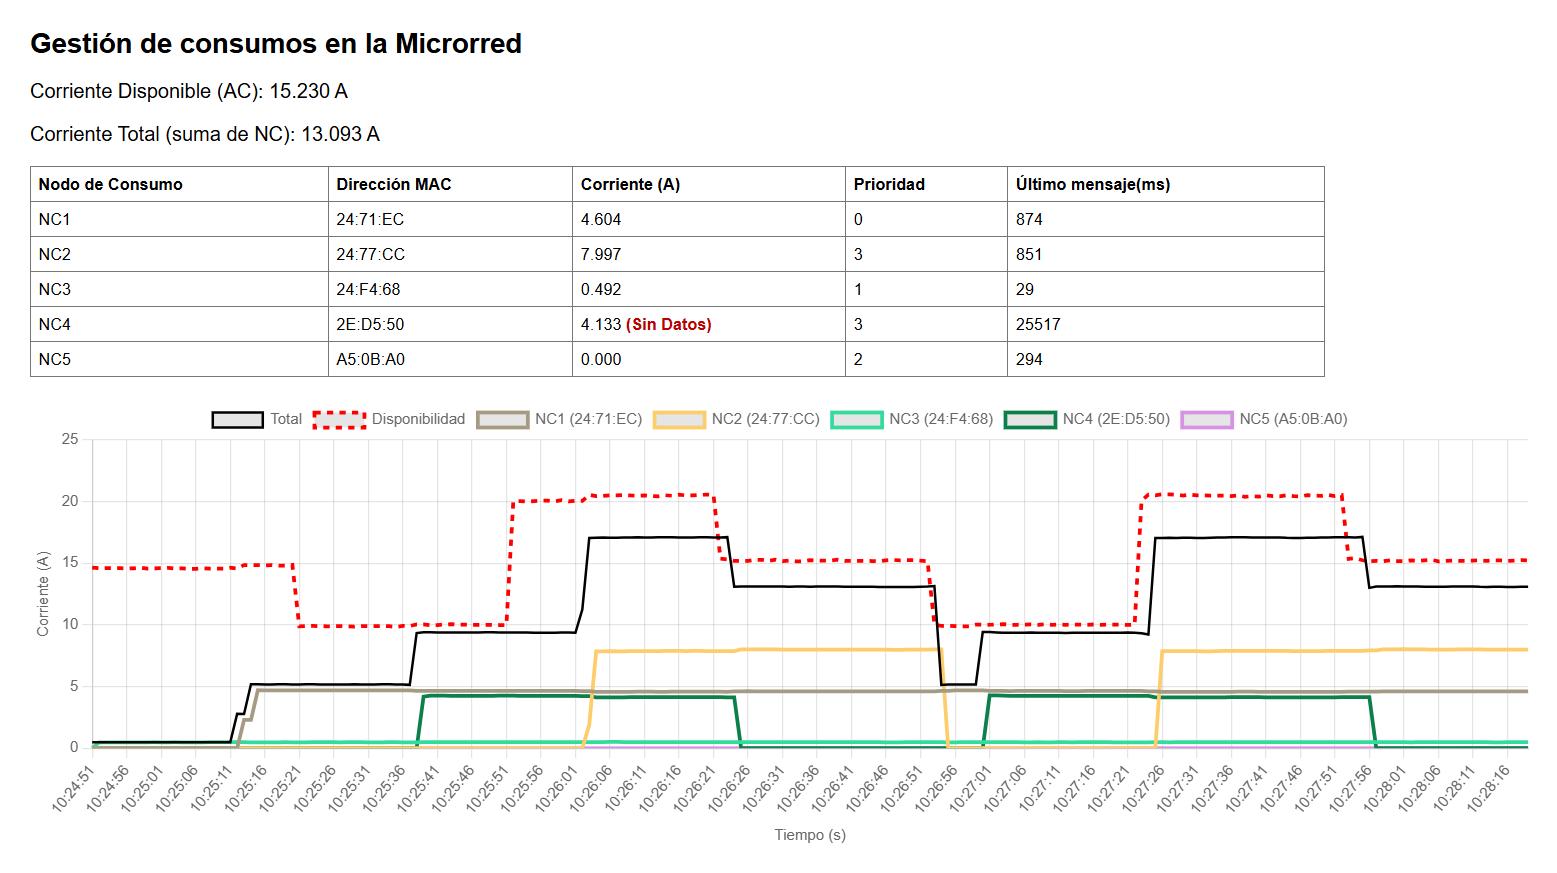
\includegraphics[width=1\textwidth]{imagenes/ensayo_carga_no_lineal.png}
    \caption{Medición de corriente en el nodo NC3 con la carga no lineal del cargador de computadora portátil.}
    \label{fig:medicion_nc3}
\end{figure}

Esta comparación permitió validar que, aun en presencia de cargas no lineales, el sistema presenta un comportamiento consistente y adecuado para medición de corriente en entornos generales.

\section{Influencia del ruido introducido por la fuente}
adasfd \dots

\section{Limitaciones del uso del protocolo ESP-NOW en conjunto con MQTT}
asda \dots
